\section{Occupation-level rents and within-group compression}
\label{sec:occupation-rents}

The family wage wedge $\omega_g$ of Section~\ref{sec:wedge} is the
geometry's counterpart to the worker rents of \textcite{acemoglu2024rents}: a
multiplicative gap between the wage a task pays and the worker's opportunity
cost, arising from the same institutional sources --- unions, licensing,
efficiency wages, bargaining, norms --- and, as there, held fixed under the
shock. With the wedge in the operated share, automation in our model targets
high-rent work: holding the technology field fixed, the displacement the wedge
\emph{adds} correlates with the rent at Spearman $+0.83$, and the
employment-weighted average rent of the surviving workforce falls
($+0.004 \to -0.055$). This reproduces the rent targeting and dissipation of
\textcite{acemoglu2024rents}, Proposition~3, as an equilibrium outcome of
cost-minimising adoption rather than an assumption.

Their second prediction --- that automation \emph{compresses} the wage
distribution \emph{within} an exposed group (Proposition~4) --- requires
within-group rent dispersion, which the family wedge, constant within a family,
does not carry. We recover it. Define the occupation rent $\eta_o$ as the
residual of the observed log wage on the occupation's priced capability content,
$\ln w_o = \beta_0 + \sum_k \beta_k\, \theta_{o,k} + \eta_o$, over the four
capabilities $\{S_1,S_2,A_1,A_2\}$. This is the wage premium that no priced
capability explains --- the occupation-level analogue of a rent --- and it is
exactly the within-family variation that the family mean of
Section~\ref{sec:wedge} discards (within-family standard deviation
$0.22$). Used as the wedge, $\eta_o$ lets automation discriminate among
occupations \emph{inside} a family.

The mechanism then operates as in \textcite{acemoglu2024rents}. Within families,
adoption targets the high-rent occupations
($\overline{\mathrm{corr}}(D_o,\eta_o) = +0.45$), and a displaced share falls
back toward its capability-determined base wage, losing the rent: the bounded
wage change is $\Delta\ln w_o = \ln[(1-D_o)e^{\eta_o} + D_o] - \eta_o \in
[-\eta_o, 0]$, larger the higher the rent
($\overline{\mathrm{corr}}(\Delta\ln w_o,\eta_o) = -0.77$). The consequence is
compression: within-family wage dispersion falls from $0.285$ to $0.251$, in
$82$ percent of families. Across the within-group wage distribution the change
traces the flat-then-falling profile of \textcite{acemoglu2024rents}, Figure~1
(Figure~\ref{fig:occupation-rents-prop4}): base-wage workers at low percentiles
are untouched, while the high-rent workers between the $70$th and the top
percentile bear the losses. The profile is a monotone hook rather than a closed
U; the up-turn at the very top in \textcite{acemoglu2024rents} arises only under
their Assumption~2(i), that the highest-rent tasks cannot be automated. Imposing
it here --- making the top five percent of rents non-automatable --- bends the
top of the profile up ($-0.13 \to -0.06$), recovering the U in direction.

The result is robust to how the rent is measured. Residualising the wage on the
single price composite (the cruder measure) attributes more of the wage to rent
($R^2 = 0.57$, against $0.66$ for the capability vector), but the targeting and
compression are essentially unchanged ($+0.44$; $86$ percent of families);
adding task-space position as a further control, which is nearly collinear with
the capabilities and raises $R^2$ by only $0.015$, also leaves them unchanged
($+0.44$; $82$ percent). Roughly ten points of what the price composite reads as
rent is in fact unmodelled capability, but the rent retains most of its
variation under the full capability control, and the within-group compression
survives. We therefore read it as a genuine implication of the geometry, not an
artefact of mismeasured rent.

Two caveats bound the claim. The rent $\eta_o$ is the entire wage residual and so
is an upper bound on the true rent: it still absorbs compensating differentials
and any capability dimension outside $\{S_1,S_2,A_1,A_2\}$, which our controls,
unlike the demographic controls of \textcite{acemoglu2024rents}, do not remove.
And the rent-loss wage change presumes, with \textcite{acemoglu2024rents}, that a
displaced high-rent worker reverts to the base wage; it is their dissipation
assumption, not an additional one, but the compression follows once high-rent
work is targeted and so is in that sense built into the mechanism rather than
independently tested. We accordingly report this as an illustration that the 2D
geometry reproduces within-group compression, not as an estimate of its
magnitude.

\begin{figure}[!htbp]
\centering
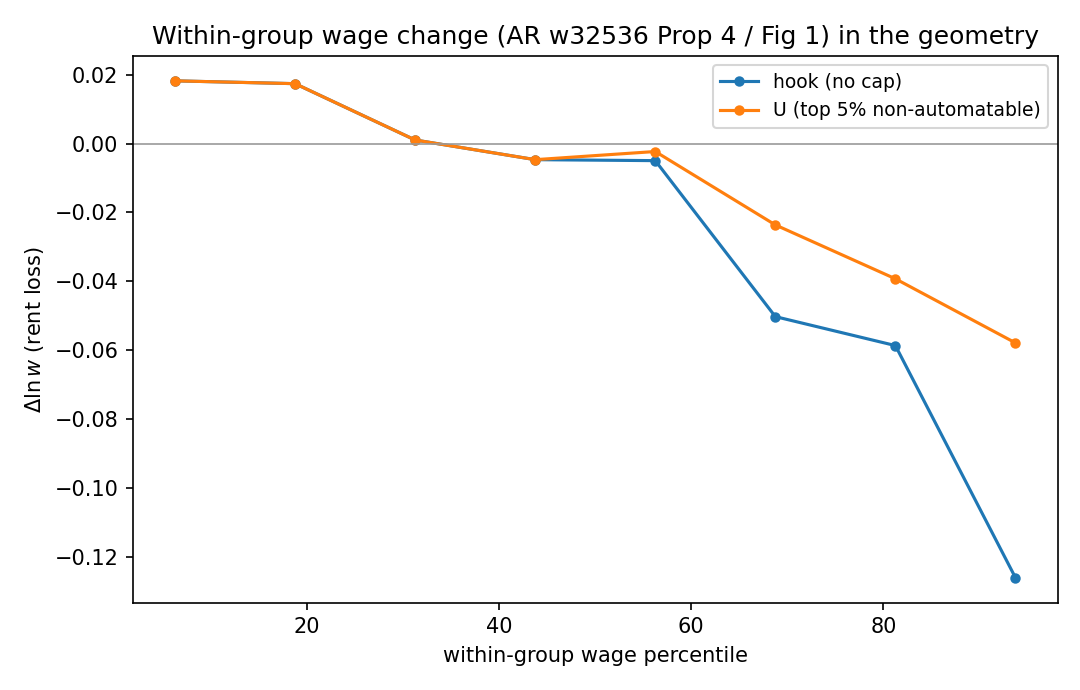
\includegraphics[width=0.72\textwidth]{occupation_rents_prop4.png}
\caption{Within-group wage change by within-group wage percentile, the geometry's
counterpart to \textcite{acemoglu2024rents}, Figure~1. Low percentiles hold
no-rent tasks and are untouched; high-rent workers above the $70$th percentile
bear the losses, compressing the within-group distribution. The hook (no cap) is
their case $\Delta\ln w_g(1) < \Delta\ln w_g$; making the highest-rent tasks
non-automatable (their Assumption~2(i)) bends the top up toward the U.}
\label{fig:occupation-rents-prop4}
\end{figure}